\documentclass{article}
\usepackage{amsmath, amsthm, amssymb, amsfonts, booktabs, hyperref, graphicx, float, esint, xcolor, subcaption, xspace}
% mathbbol, causing errors
\setlength{\abovedisplayskip}{0pt}
\setlength{\belowdisplayskip}{0pt}
\setlength{\abovedisplayshortskip}{0pt}
\setlength{\belowdisplayshortskip}{0pt}

\newcommand{\vr}{\vec{r}}
\newcommand{\vOmega}{\vec{\Omega}}
\newcommand{\vJ}{\vec{J}}
\newcommand{\vO}{\vec{\Omega}}
\newcommand{\bra}{\left\langle}
\newcommand{\ket}{\right\rangle}
\newcommand{\sbra}{\left[}
\newcommand{\sket}{\right]}
\renewcommand{\div}{\vec{\nabla} \cdot}
\newcommand{\grad}{\vec{\nabla}}
\newcommand{\vbeta}{\vec{\beta} }
\newcommand{\pdx}{\frac{\partial}{\partial x}}
\newcommand{\pdy}{\frac{\partial}{\partial y}}
\newcommand{\pdz}{\frac{\partial}{\partial z}}
\newcommand{\intrrr}{\int d^3 r \,}
\newcommand{\intrr}{\int d^2 r \,}
\newcommand{\dEdphi}{\partial_\phi E }
\newcommand{\dEdp}{\partial_p E }
\newcommand{\dBdphi}{\partial_\phi B }
\newcommand{\dBdp}{B }
\newcommand{\adj}{\phi^\dag}
\newcommand{\surf}{\int_{\partial V}}
\newcommand{\domain}{V}
\newcommand{\bound}{\partial V}
\newcommand{\vn}{\vec{n}}
\newcommand{\Edd}{\mathbb{E}}
\newcommand{\BEdd}{B}
\newcommand{\sigt}{\sigma_t}
\newcommand{\sigs}{\sigma_s}
\newcommand{\siga}{\sigma_a}
\newcommand{\isigt}{c}
% why \newcommand{\angSource}{q_\Omega}
\newcommand{\angSource}{q}
\newcommand{\scalSource}{q}
\newcommand{\angResp}{q^\dag}
\newcommand{\scalResp}{q^\dag}
\newcommand{\qoi}{{\it QoI}\xspace}


\newcommand{\comment}[2]{\marginpar{\textcolor{#2}{$\star$}}\textcolor{#2}{#1}\newline}

%-----------------------------------------------------------
%-----------------------------------------------------------
\usepackage{ifthen}
\newboolean{draftversion}
\setboolean{draftversion}{true}
%-----------------------------------------------------------
%----------------------------------------------------------

\ifthenelse{\boolean{draftversion}}
{
\newcommand{\iwh}[1]{\comment{#1}{red}}
\newcommand{\jcr}[1]{\comment{#1}{blue}}
\newcommand{\todo}[1]{\comment{#1}{purple}}
}
{
\newcommand{\iwh}[1]{\phantom{a}}
\newcommand{\jcr}[1]{\phantom{a}}
\newcommand{\todo}[1]{\phantom{a}}
}
\newcommand{\tcr}[1]{\comment{#1}{red}}

%%%%%%%%%%%%%%%%%%%%%%%%%%%%%%%%%%%%%%%%%%%%%%%%%%%%%%%%%%%%%%%%%%%%%%%%%%%%%%%%%%%%%%%%%%%%%%%%%%%%
%%%%%%%%%%%%%%%%%%%%%%%%%%%%%%%%%%%%%%%%%%%%%%%%%%%%%%%%%%%%%%%%%%%%%%%%%%%%%%%%%%%%%%%%%%%%%%%%%%%%
\begin{document}

\begin{center}
{\large Thesis Proposal~:\\
{\it Adjoint-based sensitivity for radiation transport using an Eddington tensor formulation}}\\
\vspace{2mm}
Ian Halvic, Texas A\&M University, NUEN
\end{center}

\tableofcontents
\newpage
\section{THE HOLDING PEN, DRAFT SECTION REMOVE!!!!}

\subsection{Incident Flux Through A Shield}
\begin{equation}
\phi = \phi_0 e^{\sigma_a \mu \Delta x}
\end{equation}
\begin{figure}[H]
\label{Absorber}
\centering
\begin{subfigure}{.5\textwidth}
  \centering
  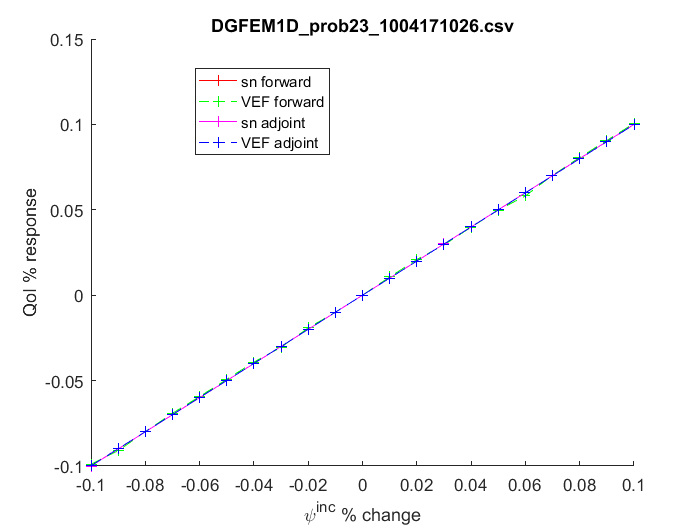
\includegraphics[width=.98\linewidth]{figures/23incSens.png}
  \caption{Unperturbed shield: $\siga=1$, $\sigs=0$. }
  \label{fig:sfig1}
\end{subfigure}%
\begin{subfigure}{.5\textwidth}
  \centering
  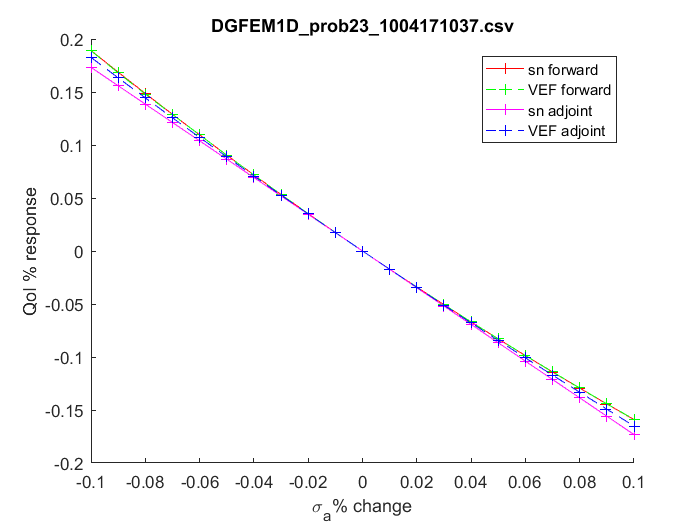
\includegraphics[width=.98\linewidth]{figures/23sigaSens.png}
  \caption{Unperturbed shield: $\siga=1$, $\sigs=0$. }
  \label{fig:sfig2}
\end{subfigure}
\end{figure}

\subsubsection{Source Through A Shield}
\begin{equation}
\phi = \phi_0 e^{\sigma_a \mu \Delta x}
\end{equation}

\begin{figure}[H]
\label{Absorber}
\centering
\begin{subfigure}{.5\textwidth}
  \centering
  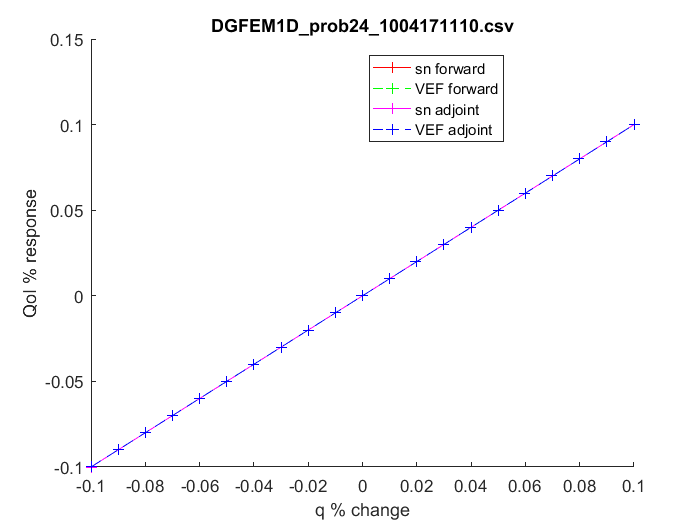
\includegraphics[width=.98\linewidth]{figures/24qSens.png}
  \caption{Unperturbed shield: $\siga=1$, $\sigs=0$. }
  \label{fig:sfig1}
\end{subfigure}%
\begin{subfigure}{.5\textwidth}
  \centering
  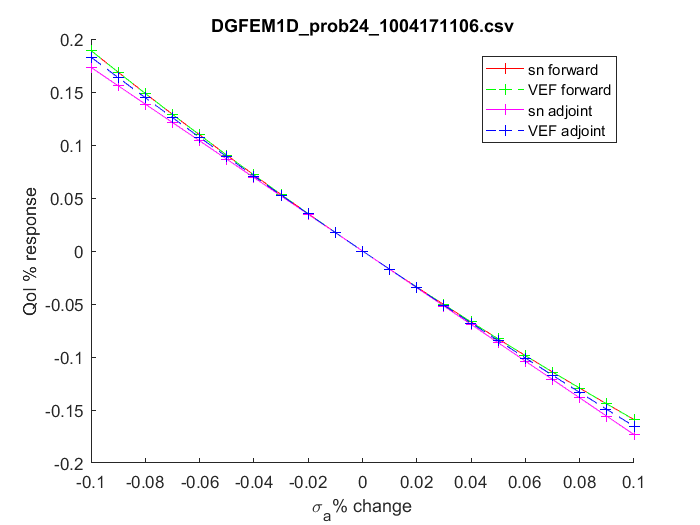
\includegraphics[width=.98\linewidth]{figures/24sigaSens.png}
  \caption{Unperturbed shield: $\siga=1$, $\sigs=0$. }
  \label{fig:sfig2}
\end{subfigure}
\end{figure}


\subsubsection{Incident Flux Through A Scatterer}

\begin{figure}[H]
\label{Scatterer}
\centering
\begin{subfigure}{.5\textwidth}
  \centering
  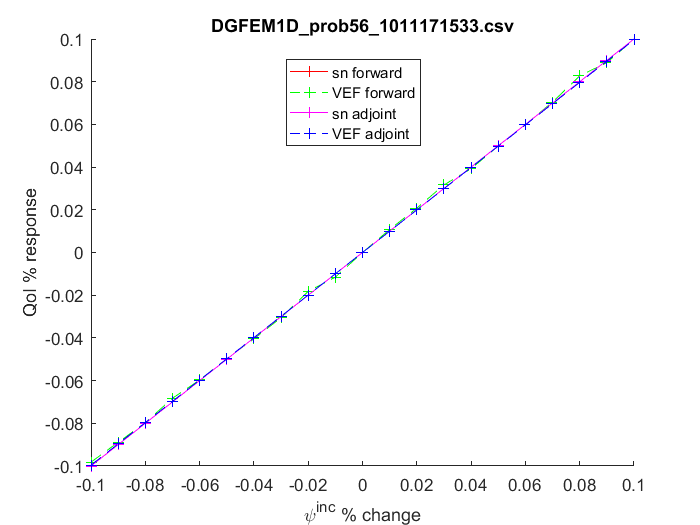
\includegraphics[width=.98\linewidth]{figures/56incSens.png}
  \caption{Unperturbed shield: $\siga=0$, $\sigs=1$. }
  \label{fig:sfig1}
\end{subfigure}%
\begin{subfigure}{.5\textwidth}
  \centering
  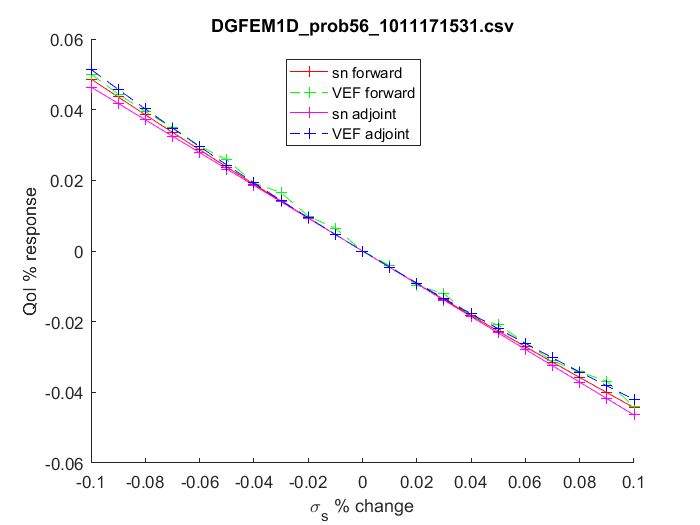
\includegraphics[width=.98\linewidth]{figures/56sigsSens.png}
  \caption{Unperturbed shield: $\siga=0$, $\sigs=1$. }
  \label{fig:sfig2}
\end{subfigure}
\end{figure}

\subsubsection{Incident Flux Through A Scatterer into Absorber}

\begin{figure}[H]
\label{Scatterer}
\centering
\begin{subfigure}{.5\textwidth}
  \centering
  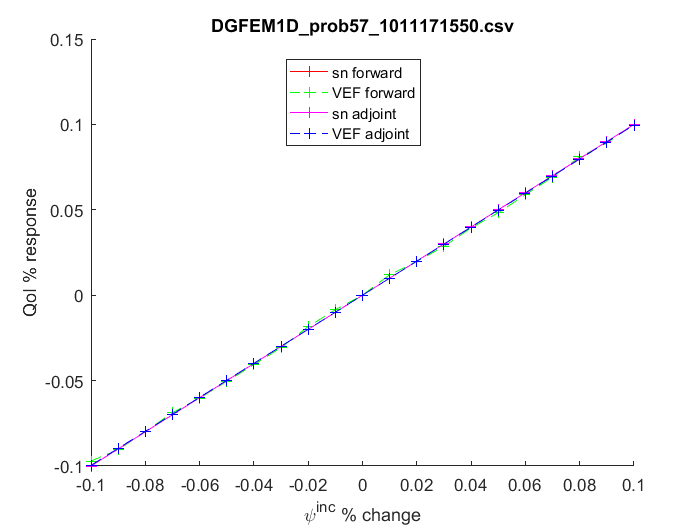
\includegraphics[width=.98\linewidth]{figures/57incSens.png}
  \caption{Unperturbed shield: $\siga=0.1$, $\sigs=1$. }
  \label{fig:sfig1}
\end{subfigure}%
\begin{subfigure}{.5\textwidth}
  \centering
  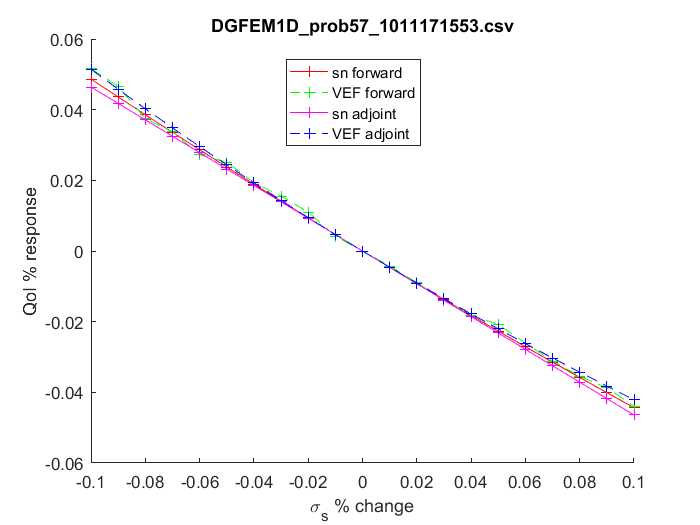
\includegraphics[width=.98\linewidth]{figures/57sigsSens.png}
  \caption{Unperturbed shield: $\siga=0.1$, $\sigs=1$. }
  \label{fig:sfig2}
\end{subfigure}
\end{figure}

%%%%%%%%%%%%%%%%%%%%%%%%%%%%%%%%%%%%%%%%%%%%%%%%%%%%%%%%%%%%%
\subsection{Simple Cases}
%%%%%%%%%%%%%%%%%%%%%%%%%%%%%%%%%%%%%%%%%%%%%%%%%%%%%%%%%%%%
%%----------------------------------------------------------------------------------------------
\subsubsection{Homogeneous System, Uniform Perturbations}
%%%%%%%----------------------------------------------------------------------------------------------
Test case consisting of a 1D homogeneous system, with a volumetric source throughout. The width of the system was 10 (arbitrary units). Solutions were obtained using a 200 element mesh. Three systems of varying initial cross sections $\sigt$ and $\sigs$ were tested. Perturbations in $\sigt$, $\sigs$, and $\scalSource$ to the system were made uniformly, resulting in the perturbed system remaining homogeneous. The desired \qoi is the total flux in the middle fifth of the system.

\todo{Add in incident flux perturbations. In the unperturbed state, the incident flux is 0, so we cant use a \% perturbation and will instead have to opt for an absolute perturbation}

\jcr{change the other figures/caption in the same manner}

\begin{figure}[H]
\label{HomoPerts}
\centering
\begin{subfigure}{.5\textwidth}
  \centering
  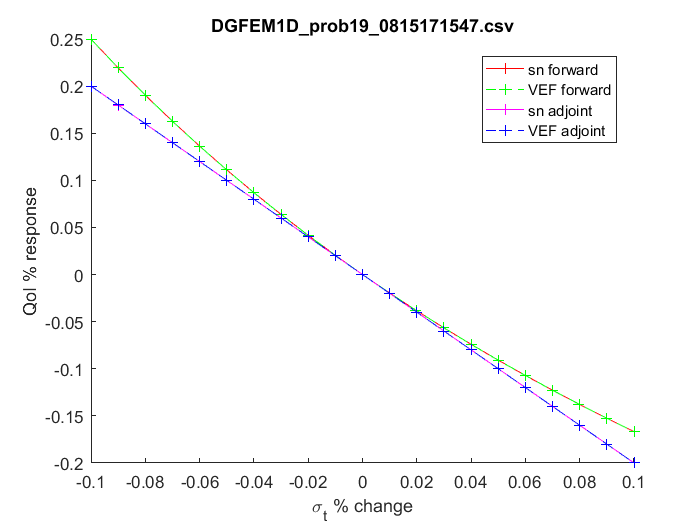
\includegraphics[width=.98\linewidth]{figures/19sigtSens.png}
  \caption{Unperturbed state: $\sigt=2$, $\sigs=1$.}
  \label{fig:sfig1}
\end{subfigure}%
\begin{subfigure}{.5\textwidth}
  \centering
  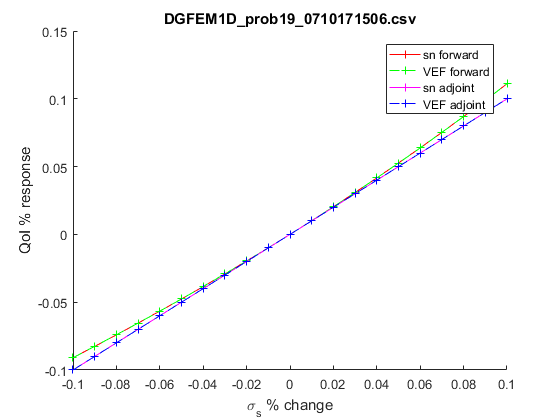
\includegraphics[width=.98\linewidth]{figures/19sigsSens.png}
  \caption{Unperturbed state: $\sigt=2$, $\sigs=1$.}
  \label{fig:sfig4}
\end{subfigure}%
\\
\begin{subfigure}{.5\textwidth}
  \centering
  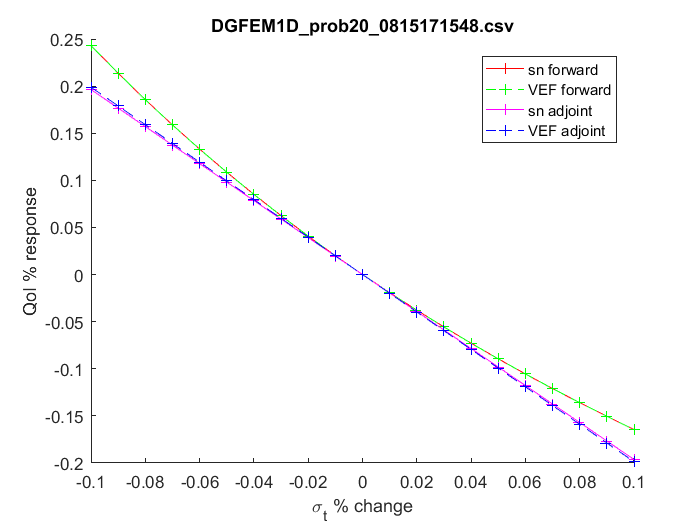
\includegraphics[width=.98\linewidth]{figures/20sigtSens.png}
  \caption{Unperturbed state: $\sigt=1$, $\sigs=0.5$.}
  \label{fig:sfig2}
\end{subfigure}%
\begin{subfigure}{.5\textwidth}
  \centering
  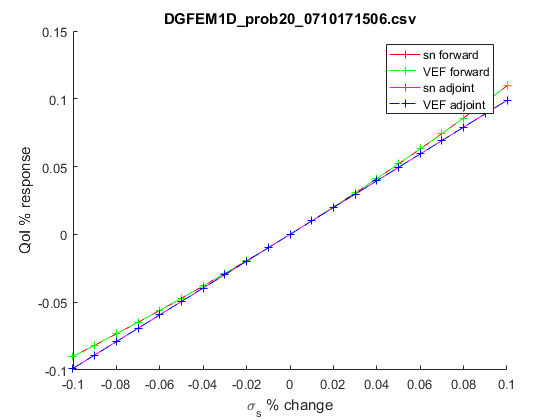
\includegraphics[width=.98\linewidth]{figures/20sigsSens.png}
  \caption{Unperturbed state: $\sigt=1$, $\sigs=0.5$.}
  \label{fig:sfig5}
\end{subfigure}%
\\
\begin{subfigure}{.5\textwidth}
  \centering
  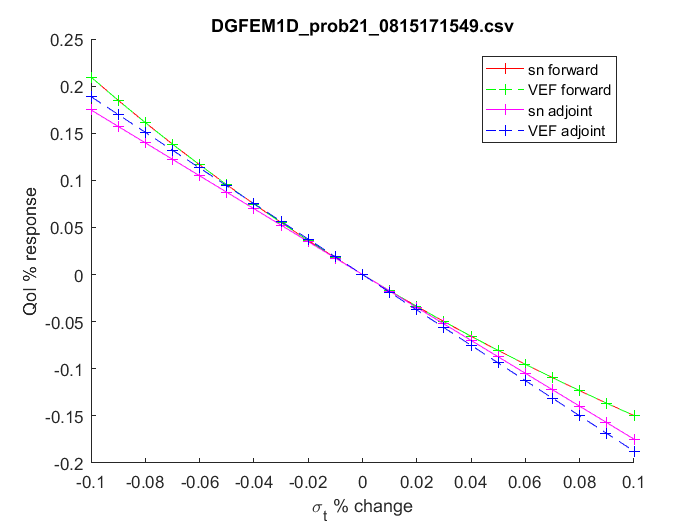
\includegraphics[width=.98\linewidth]{figures/21sigtSens.png}
  \caption{Unperturbed state: $\sigt=0.5$, $\sigs=0.25$.}
  \label{fig:sfig3}
\end{subfigure}%
\begin{subfigure}{.5\textwidth}
  \centering
  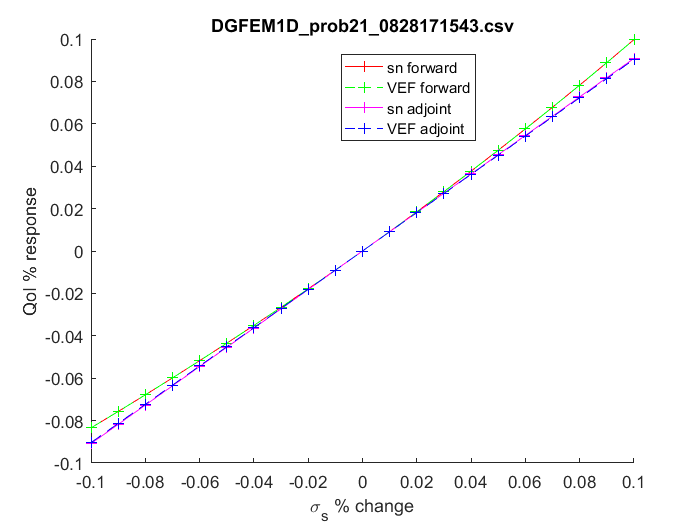
\includegraphics[width=.98\linewidth]{figures/21sigsSens.png}
  \caption{Unperturbed state: $\sigt=0.5$, $\sigs=0.25$.}
  \label{fig:sfig6}
\end{subfigure}%
\caption{Plots of $\sigt$ and $\sigs$ perturbation sensitivity for uniformly perturbed system.}
\label{fig:fig}
\end{figure}

\begin{figure}[H]
\label{HomoPertq}
\centering
\begin{subfigure}{.5\textwidth}
  \centering
  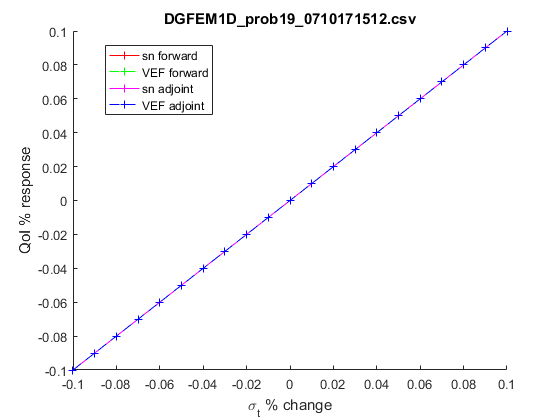
\includegraphics[width=.98\linewidth]{figures/19qSens.png}
  \caption{Unperturbed state: $\sigt=2$, $\sigs=1$}
  \label{fig:sfig1}
\end{subfigure}%
\begin{subfigure}{.5\textwidth}
  \centering
  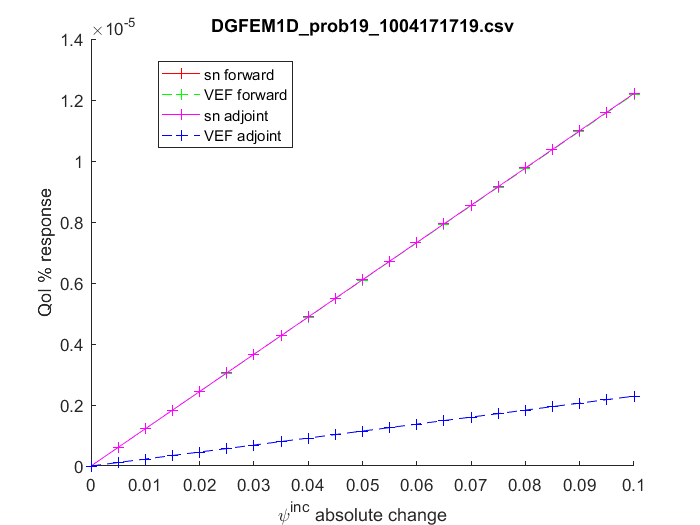
\includegraphics[width=.98\linewidth]{figures/19incSens.png}
  \caption{Unperturbed state: $\sigt=2$, $\sigs=1$}
  \label{fig:sfig4}
\end{subfigure}%
\\
\begin{subfigure}{.5\textwidth}
  \centering
  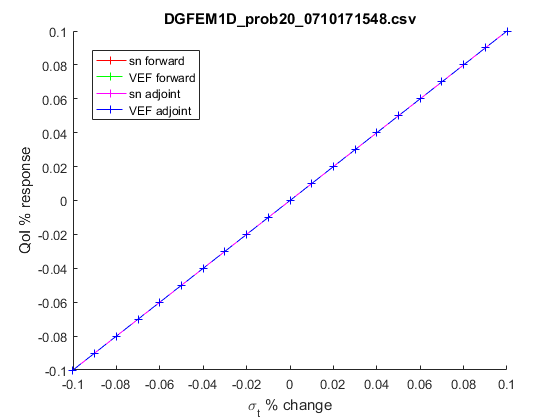
\includegraphics[width=.98\linewidth]{figures/20qSens.png}
  \caption{Unperturbed state: $\sigt=1$, $\sigs=0.5$}
  \label{fig:sfig2}
\end{subfigure}%
\begin{subfigure}{.5\textwidth}
  \centering
  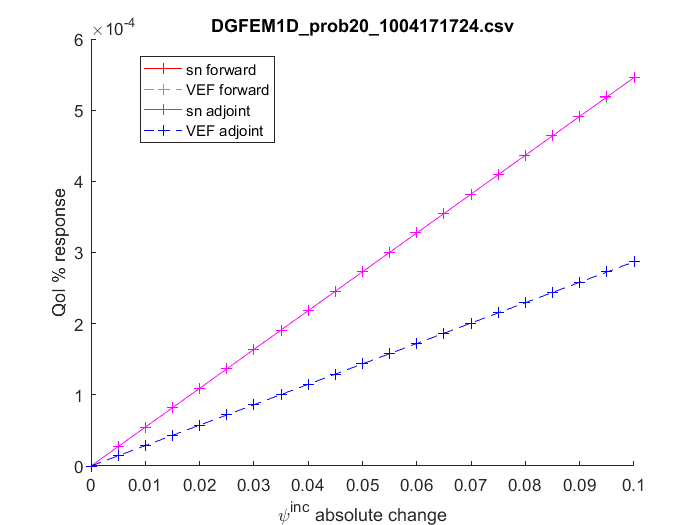
\includegraphics[width=.98\linewidth]{figures/20incSens.png}
  \caption{Unperturbed state: $\sigt=1$, $\sigs=0.5$}
  \label{fig:sfig5}
\end{subfigure}%
\\
\begin{subfigure}{.5\textwidth}
  \centering
  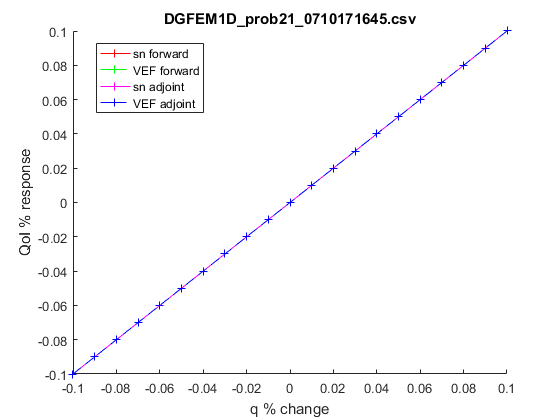
\includegraphics[width=.98\linewidth]{figures/21qSens.png}
  \caption{Unperturbed state: $\sigt=0.5$, $\sigs=0.25$}
  \label{fig:sfig3}
\end{subfigure}%
\begin{subfigure}{.5\textwidth}
  \centering
  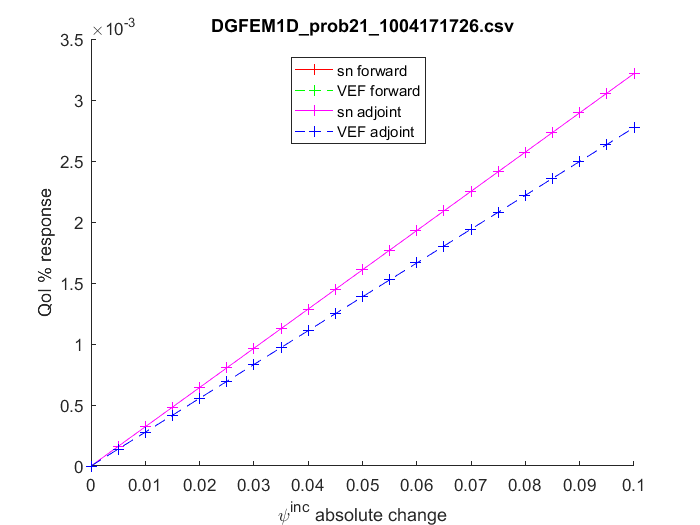
\includegraphics[width=.98\linewidth]{figures/21incSens.png}
  \caption{Unperturbed state: $\sigt=0.5$, $\sigs=0.25$}
  \label{fig:sfig6}
\end{subfigure}%
\caption{Plots of source and incident flux perturbation sensitivities for uniformly perturbed system.}
\label{fig:fig}
\end{figure}

\jcr{comment the results!}

\jcr{why no examples with changing the incident flux value?}



\subsubsection{Region boundary perturbation}
\begin{figure}[H]
\label{Boundaries}
\centering
\begin{subfigure}{.5\textwidth}
  \centering
  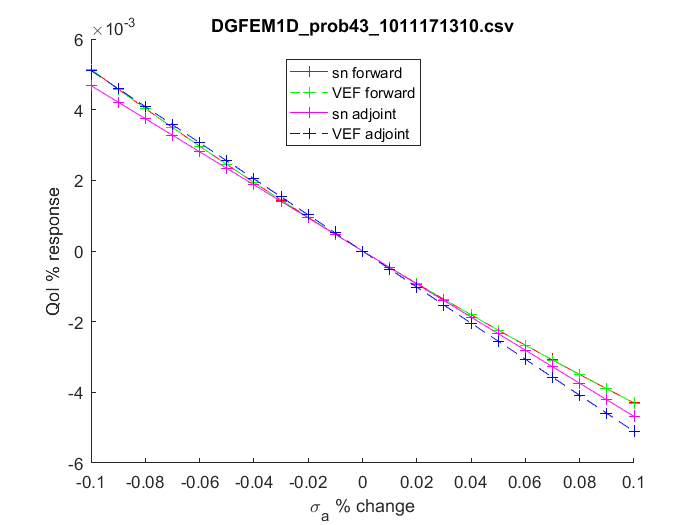
\includegraphics[width=.98\linewidth]{figures/43sigaSens.png}
  \caption{QoI outside}
  \label{fig:sfig1}
\end{subfigure}%
\begin{subfigure}{.5\textwidth}
  \centering
  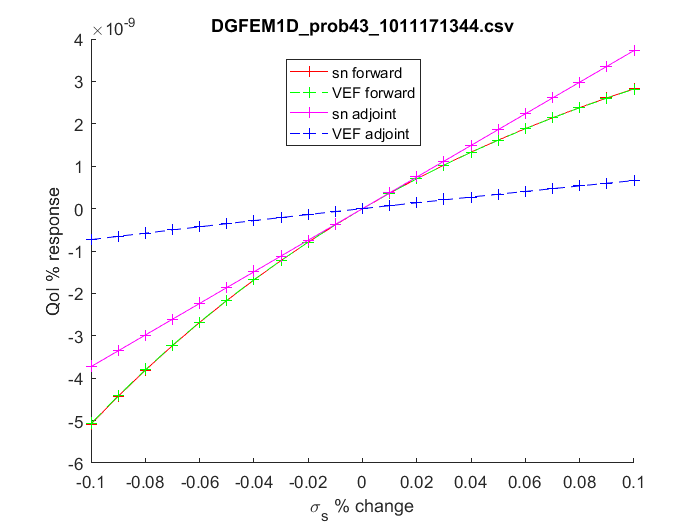
\includegraphics[width=.98\linewidth]{figures/43sigsSens.png}
  \caption{QoI outside}
  \label{fig:sfig4}
\end{subfigure}%
\\
\begin{subfigure}{.5\textwidth}
  \centering
  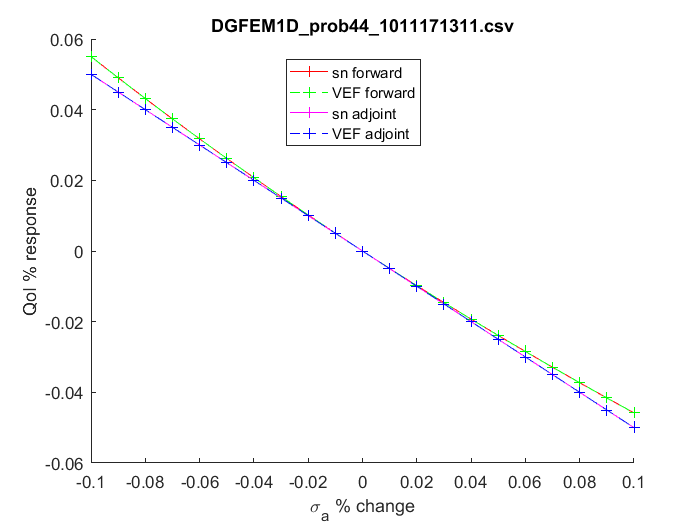
\includegraphics[width=.98\linewidth]{figures/44sigaSens.png}
  \caption{centered QoI}
  \label{fig:sfig2}
\end{subfigure}%
\begin{subfigure}{.5\textwidth}
  \centering
  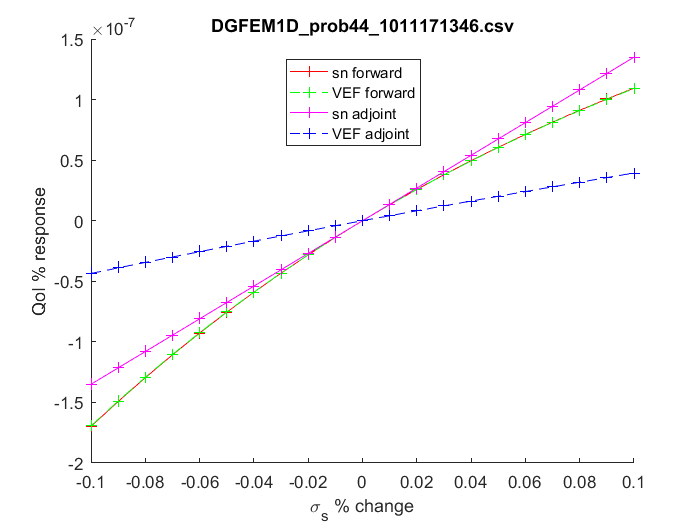
\includegraphics[width=.98\linewidth]{figures/44sigsSens.png}
  \caption{centered QoI}
  \label{fig:sfig5}
\end{subfigure}%
\\
\begin{subfigure}{.5\textwidth}
  \centering
  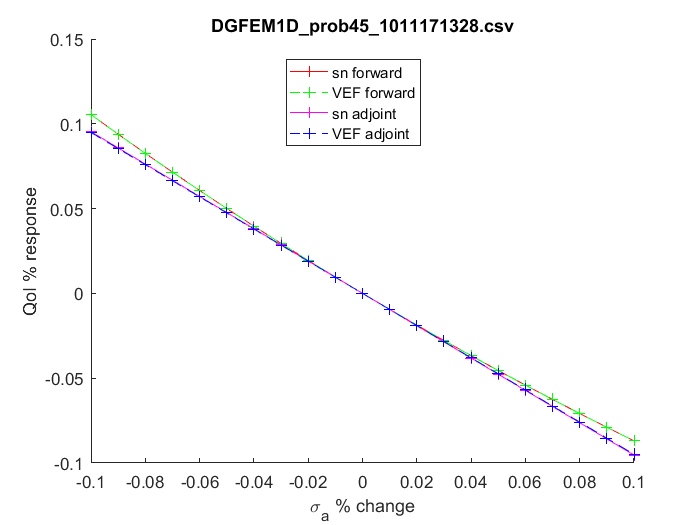
\includegraphics[width=.98\linewidth]{figures/45sigaSens.png}
  \caption{QoI inside Pert}
  \label{fig:sfig3}
\end{subfigure}%
\begin{subfigure}{.5\textwidth}
  \centering
  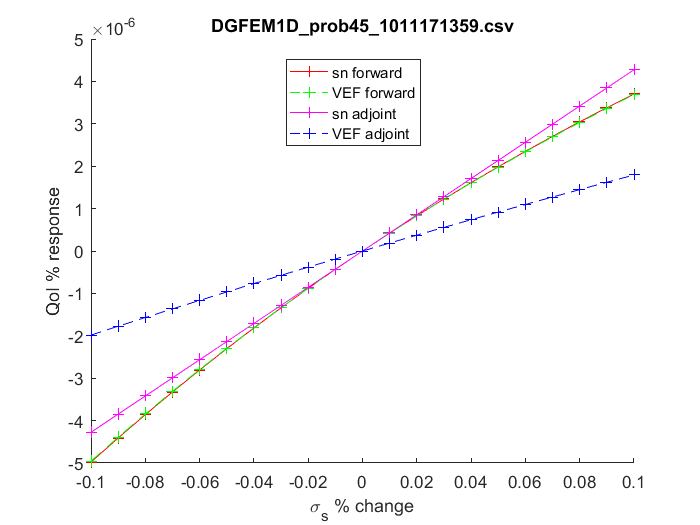
\includegraphics[width=.98\linewidth]{figures/45sigsSens.png}
  \caption{QoI inside pert}
  \label{fig:sfig6}
\end{subfigure}%
\caption{Plots of various qoi to layer perturbation system. Initial is homogeneous $\siga=1$ and $sigs=1$.}
\label{fig:fig}
\end{figure}

%%%%%%%----------------------------------------------------------------------------------------------
\subsection{Homogeneous initial system, Non-Uniform Perturbations}
%%%%%%%----------------------------------------------------------------------------------------------

The next test case has the same initial conditions as the previous homogeneous case. however the system is perturbed into a inhomogeneous system. The system is split into 5 equal widths. The first, third, and fifth sections (corresponding to the center and the end sections) have the relevant variable perturbed in one direction, while the other two segments are perturbed in the opposite direction. The result is a system that is inhomogeneous, but with regular variations and symmetric about the midpoint. The \qoi is also retained from the previous case.

\jcr{change the other figures/caption in the same manner as before}

\begin{figure}[H]
\label{InHomoPertt}
\centering
\begin{subfigure}{.5\textwidth}
  \centering
  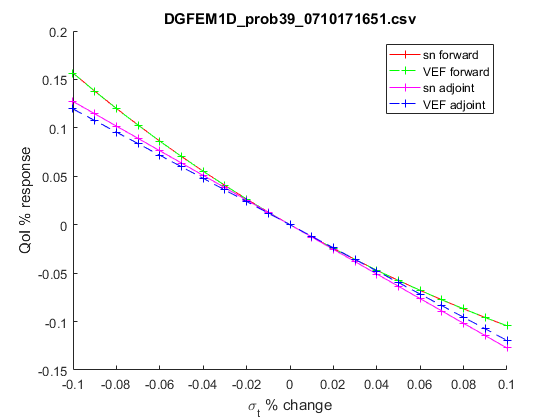
\includegraphics[width=.98\linewidth]{figures/39sigtSens.png}
  \caption{Unperturbed state: $\sigt=2$, $\sigs=1$.}
  \label{fig:sfig1}
\end{subfigure}%
\begin{subfigure}{.5\textwidth}
  \centering
  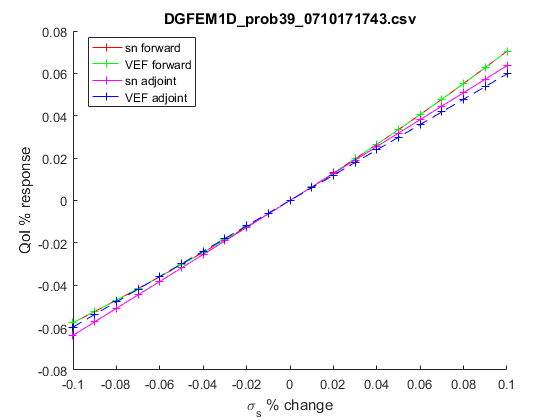
\includegraphics[width=.98\linewidth]{figures/39sigsSens.png}
  \caption{Unperturbed state: $\sigt=2$, $\sigs=1$.}
  \label{fig:sfig4}
\end{subfigure}%
\\
\begin{subfigure}{.5\textwidth}
  \centering
  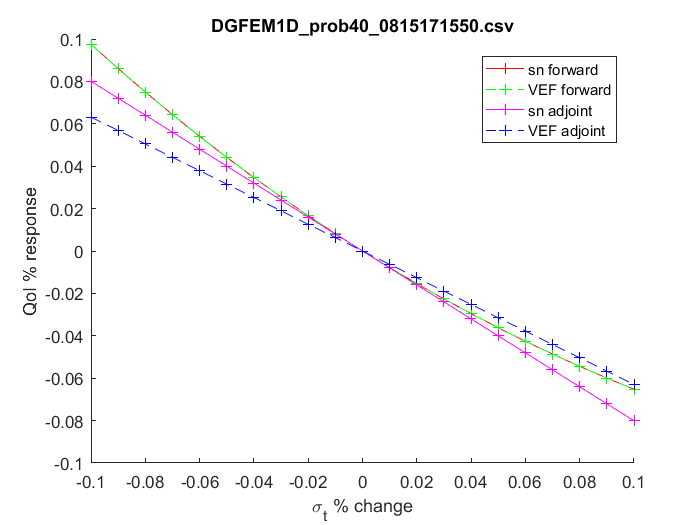
\includegraphics[width=.98\linewidth]{figures/40sigtSens.png}
  \caption{Unperturbed state: $\sigt=1$, $\sigs=0.5$.}
  \label{fig:sfig2}
\end{subfigure}%
\begin{subfigure}{.5\textwidth}
  \centering
  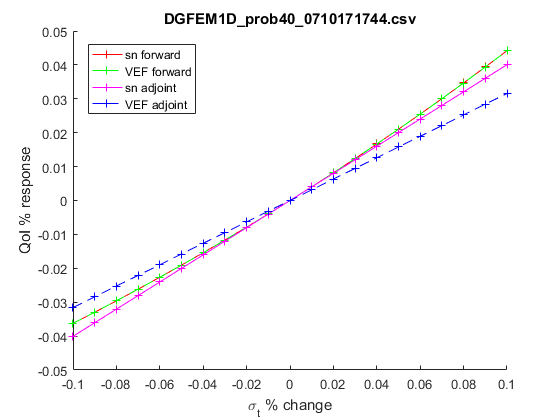
\includegraphics[width=.98\linewidth]{figures/40sigsSens.png}
  \caption{Unperturbed state: $\sigt=1$, $\sigs=0.5$.}
  \label{fig:sfig5}
\end{subfigure}%
\\
\begin{subfigure}{.5\textwidth}
  \centering
  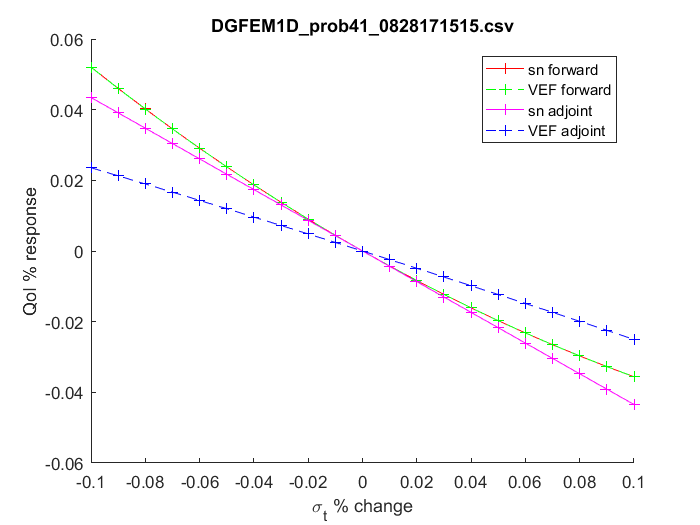
\includegraphics[width=.98\linewidth]{figures/41sigtSens.png}
  \caption{Unperturbed state: $\sigt=0.5$, $\sigs=0.25$.}
  \label{fig:sfig3}
\end{subfigure}%
\begin{subfigure}{.5\textwidth}
  \centering
  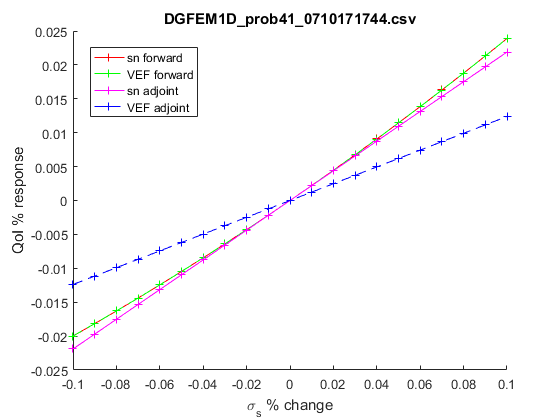
\includegraphics[width=.98\linewidth]{figures/41sigsSens.png}
  \caption{Unperturbed state: $\sigt=0.5$, $\sigs=0.25$.}
  \label{fig:sfig6}
\end{subfigure}%
\caption{Plots of $\siga$ and $\sigs$ perturbation sensitivity for non-uniformly perturbed system.}
\label{fig:fig}
\end{figure}

\begin{figure}[H]
\label{InHomoPertq}
\centering
\begin{subfigure}{.5\textwidth}
  \centering
  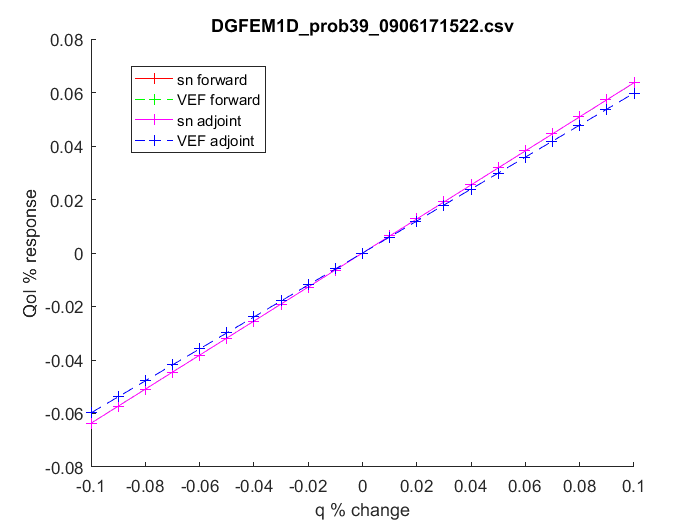
\includegraphics[width=.98\linewidth]{figures/39qSens.png}
  \caption{Unperturbed state: $\sigt=2$, $\sigs=1$}
  \label{fig:sfig1}
\end{subfigure}%
\begin{subfigure}{.5\textwidth}
  \centering
  
\includegraphics[width=.98\linewidth]{figures/holder.png}
  \caption{Unperturbed state: $\sigt=2$, $\sigs=1$}
  \label{fig:sfig4}
\end{subfigure}%
\\
\begin{subfigure}{.5\textwidth}
  \centering
  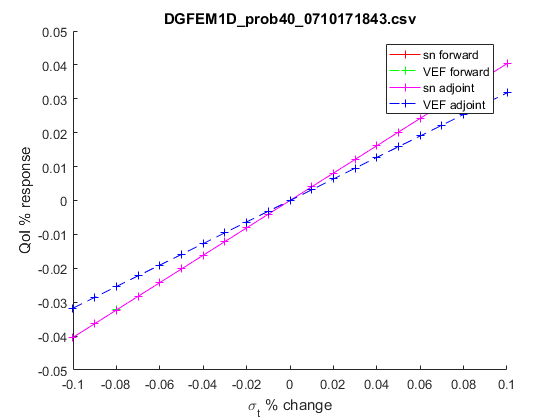
\includegraphics[width=.98\linewidth]{figures/40qSens.png}
  \caption{Unperturbed state: $\sigt=1$, $\sigs=0.5$}
  \label{fig:sfig2}
\end{subfigure}%
\begin{subfigure}{.5\textwidth}
  \centering
  
\includegraphics[width=.98\linewidth]{figures/holder.png}
  \caption{Unperturbed state: $\sigt=1$, $\sigs=0.5$}
  \label{fig:sfig5}
\end{subfigure}%
\\
\begin{subfigure}{.5\textwidth}
  \centering
  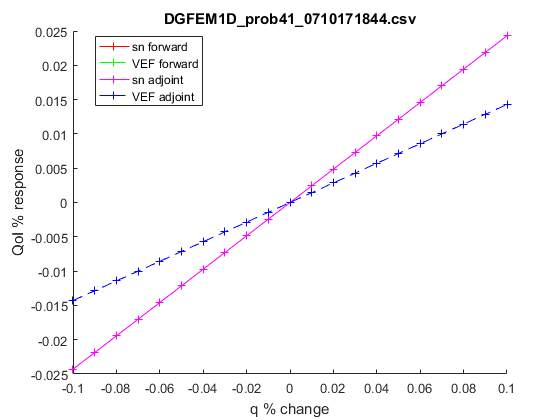
\includegraphics[width=.98\linewidth]{figures/41qSens.png}
  \caption{Unperturbed state: $\sigt=0.5$, $\sigs=0.25$}
  \label{fig:sfig3}
\end{subfigure}%
\begin{subfigure}{.5\textwidth}
  \centering
  
\includegraphics[width=.98\linewidth]{figures/holder.png}
  \caption{Unperturbed state: $\sigt=0.5$, $\sigs=0.25$}
  \label{fig:sfig6}
\end{subfigure}%
\caption{Plots of source ans incident perturbation sensitivities for non-uniformly perturbed system.}
\label{fig:fig}
\end{figure}


\jcr{comment the results!}

\jcr{why no examples with changing the incident flux value?}

%%%%%%%----------------------------------------------------------------------------------------------
\subsubsection{Streaming system}
%%%%%%%----------------------------------------------------------------------------------------------
To generate a streaming system, we retain the 5 equal width sectioning of the previous inhomogeneous example, but the second and fourth sections are converted to streaming regions ($\sigt \approx 0 $). Leaving three neutron producing sections separated by two streaming gaps. The \qoi remains as the total neutron count in the center fifth section.

\jcr{same comments as above}
\todo{Add in incident flux perturbation cases, similar to the homogeneous case.}

\begin{figure}[H]
\label{Streaming}
\centering
\begin{subfigure}{.5\textwidth}
  \centering
  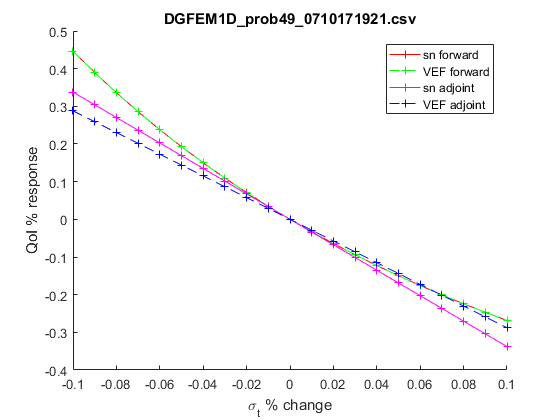
\includegraphics[width=.98\linewidth]{figures/49sigtSens.png}
  \caption{Unperturbed state: $\sigt=2$, $\sigs=1$.}
  \label{fig:sfig1}
\end{subfigure}%
\begin{subfigure}{.5\textwidth}
  \centering
  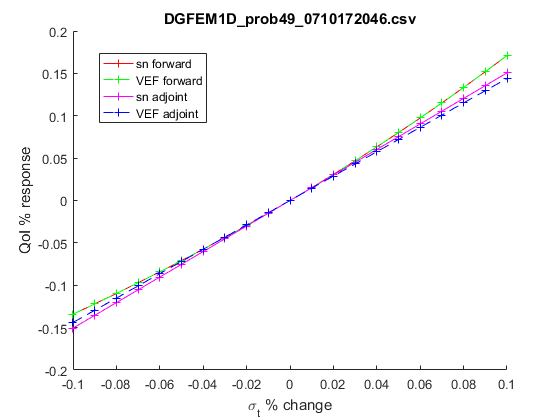
\includegraphics[width=.98\linewidth]{figures/49sigsSens.png}
  \caption{Unperturbed state: $\sigt=2$, $\sigs=1$.}
  \label{fig:sfig4}
\end{subfigure}%
\\
\begin{subfigure}{.5\textwidth}
  \centering
  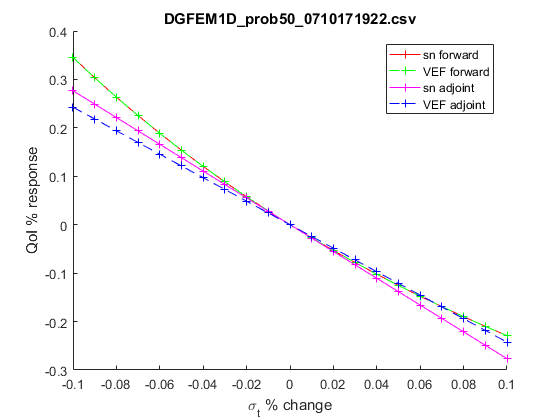
\includegraphics[width=.98\linewidth]{figures/50sigtSens.png}
  \caption{Unperturbed state: $\sigt=1$, $\sigs=0.5$.}
  \label{fig:sfig2}
\end{subfigure}%
\begin{subfigure}{.5\textwidth}
  \centering
  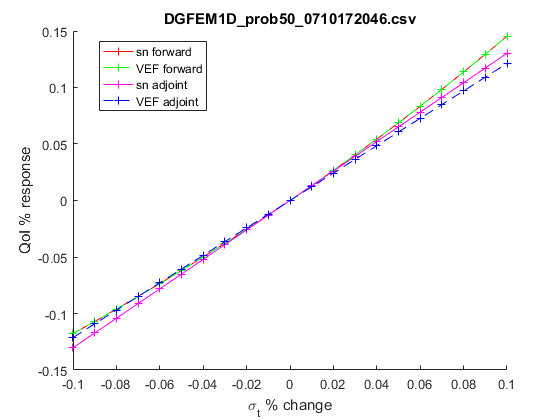
\includegraphics[width=.98\linewidth]{figures/50sigsSens.png}
  \caption{Unperturbed state: $\sigt=1$, $\sigs=0.5$.}
  \label{fig:sfig5}
\end{subfigure}%
\\
\begin{subfigure}{.5\textwidth}
  \centering
  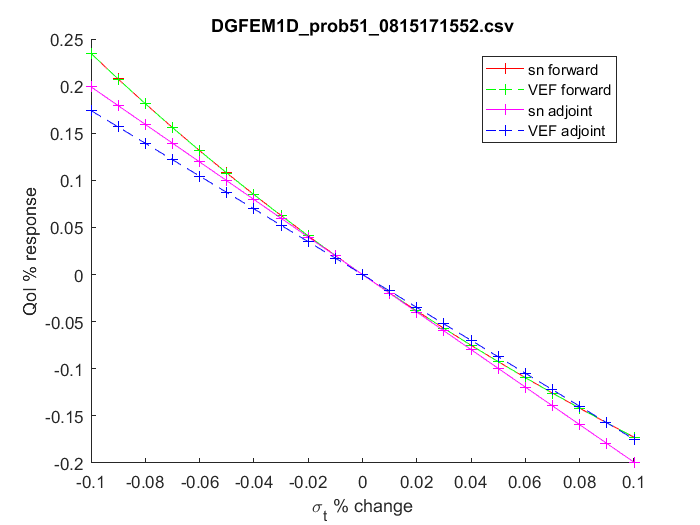
\includegraphics[width=.98\linewidth]{figures/51sigtSens.png}
  \caption{Unperturbed state: $\sigt=0.5$, $\sigs=0.25$.}
  \label{fig:sfig3}
\end{subfigure}%
\begin{subfigure}{.5\textwidth}
  \centering
  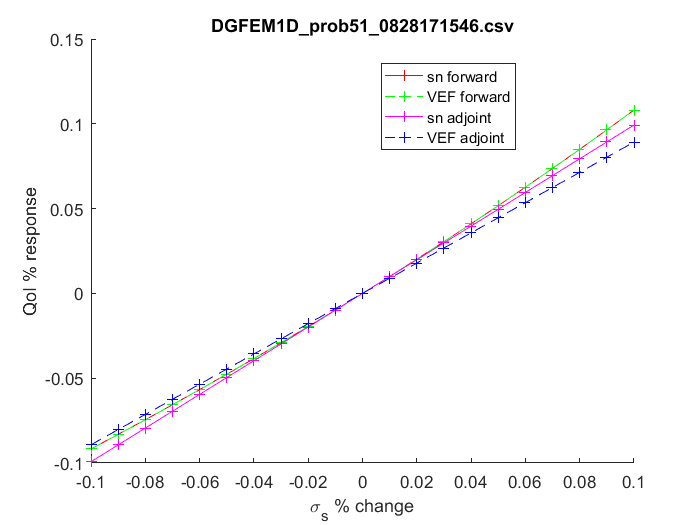
\includegraphics[width=.98\linewidth]{figures/51sigsSens.png}
  \caption{Unperturbed state: $\sigt=0.5$, $\sigs=0.25$.}
  \label{fig:sfig6}
\end{subfigure}%
\caption{Plots of $\sigt$ perturbation sensitivity for perturbed streaming system.}
\label{fig:fig}
\end{figure}


\begin{figure}[H]
\label{InHomoPertq}
\centering
\begin{subfigure}{.5\textwidth}
  \centering
  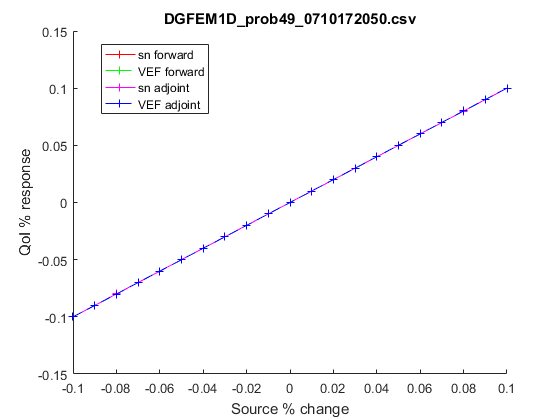
\includegraphics[width=.98\linewidth]{figures/49qSens.png}
  \caption{Unperturbed state: $\sigt=2$, $\sigs=1$}
  \label{fig:sfig1}
\end{subfigure}%
\begin{subfigure}{.5\textwidth}
  \centering
  
\includegraphics[width=.98\linewidth]{figures/holder.png}
  \caption{Unperturbed state: $\sigt=2$, $\sigs=1$}
  \label{fig:sfig4}
\end{subfigure}%
\\
\begin{subfigure}{.5\textwidth}
  \centering
  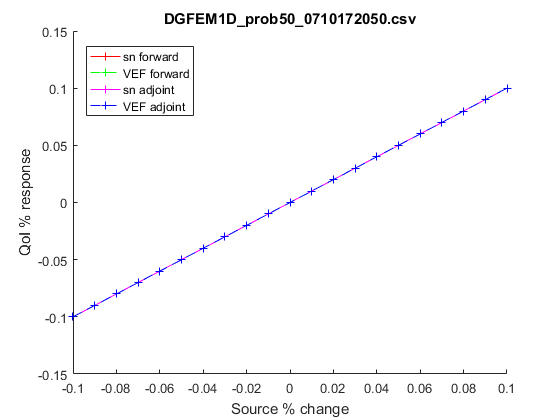
\includegraphics[width=.98\linewidth]{figures/50qSens.png}
  \caption{Unperturbed state: $\sigt=1$, $\sigs=0.5$}
  \label{fig:sfig2}
\end{subfigure}%
\begin{subfigure}{.5\textwidth}
  \centering
  
\includegraphics[width=.98\linewidth]{figures/holder.png}
  \caption{Unperturbed state: $\sigt=1$, $\sigs=0.5$}
  \label{fig:sfig5}
\end{subfigure}%
\\
\begin{subfigure}{.5\textwidth}
  \centering
  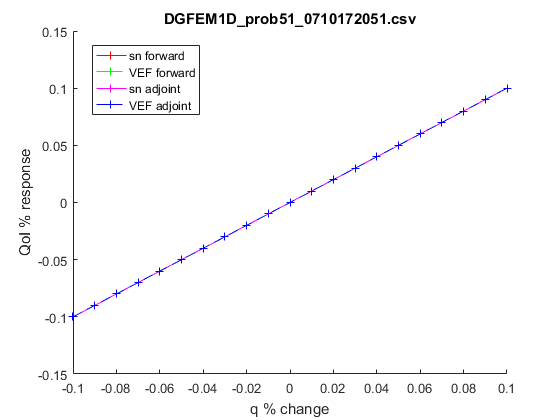
\includegraphics[width=.98\linewidth]{figures/51qSens.png}
  \caption{Unperturbed state: $\sigt=0.5$, $\sigs=0.25$}
  \label{fig:sfig3}
\end{subfigure}%
\begin{subfigure}{.5\textwidth}
  \centering
  
\includegraphics[width=.98\linewidth]{figures/holder.png}
  \caption{Unperturbed state: $\sigt=0.5$, $\sigs=0.25$}
  \label{fig:sfig6}
\end{subfigure}%
\caption{Plots of source perturbation sensitivity for perturbed streaming system.}
\label{fig:fig}
\end{figure}


%%%%%%%%%%%%%%%%%%%%%%%%%%%%%%%%%%%%%%%%%%%%%%%%%%%%%%%%%%%%
\subsection{Complex systems}
%%%%%%%%%%%%%%%%%%%%%%%%%%%%%%%%%%%%%%%%%%%%%%%%%%%%%%%%%%%%
\subsubsection{Reed Problem}

\begin{figure}[H]
\label{Streaming}
\centering
\begin{subfigure}{.5\textwidth}
  \centering
  \includegraphics[width=.98\linewidth]{figures/7sigaSens.png}
  \caption{Unperturbed state:}
  \label{fig:sfig1}
\end{subfigure}%
\begin{subfigure}{.5\textwidth}
  \centering
  \includegraphics[width=.98\linewidth]{figures/7sigsSens.png}
  \caption{Unperturbed state:}
  \label{fig:sfig4}
\end{subfigure}%
\\
\begin{subfigure}{.5\textwidth}
  \centering
  \includegraphics[width=.98\linewidth]{figures/holder.png}
  \caption{Unperturbed state:}
  \label{fig:sfig2}
\end{subfigure}%
\begin{subfigure}{.5\textwidth}
  \centering
  \includegraphics[width=.98\linewidth]{figures/holder.png}
  \caption{Unperturbed state:}
  \label{fig:sfig5}
\end{subfigure}%
\\
\begin{subfigure}{.5\textwidth}
  \centering
  \includegraphics[width=.98\linewidth]{figures/holder.png}
  \caption{Unperturbed state:}
  \label{fig:sfig3}
\end{subfigure}%
\begin{subfigure}{.5\textwidth}
  \centering
  \includegraphics[width=.98\linewidth]{figures/holder.png}
  \caption{Unperturbed state:}
  \label{fig:sfig6}
\end{subfigure}%
\caption{Sigma perturbations Reed problem}
\label{fig:fig}
\end{figure}


\begin{figure}[H]
\label{InHomoPertq}
\centering
\begin{subfigure}{.5\textwidth}
  \centering
  \includegraphics[width=.98\linewidth]{figures/7qSens.png}
  \caption{Unperturbed state: $\sigt=2$, $\sigs=1$}
  \label{fig:sfig1}
\end{subfigure}%
\begin{subfigure}{.5\textwidth}
  \centering
  \includegraphics[width=.98\linewidth]{figures/holder.png}
  \caption{Unperturbed state: $\sigt=2$, $\sigs=1$}
  \label{fig:sfig4}
\end{subfigure}%
\\
\begin{subfigure}{.5\textwidth}
  \centering
  \includegraphics[width=.98\linewidth]{figures/holder.png}
  \caption{Unperturbed state: $\sigt=1$, $\sigs=0.5$}
  \label{fig:sfig2}
\end{subfigure}%
\begin{subfigure}{.5\textwidth}
  \centering
  \includegraphics[width=.98\linewidth]{figures/holder.png}
  \caption{Unperturbed state: $\sigt=1$, $\sigs=0.5$}
  \label{fig:sfig5}
\end{subfigure}%
\\
\begin{subfigure}{.5\textwidth}
  \centering
  \includegraphics[width=.98\linewidth]{figures/holder.png}
  \caption{Unperturbed state: $\sigt=0.5$, $\sigs=0.25$}
  \label{fig:sfig3}
\end{subfigure}%
\begin{subfigure}{.5\textwidth}
  \centering
  \includegraphics[width=.98\linewidth]{figures/holder.png}
  \caption{Unperturbed state: $\sigt=0.5$, $\sigs=0.25$}
  \label{fig:sfig6}
\end{subfigure}%
\caption{Plots of source perturbation sensitivity for perturbed streaming system.}
\label{fig:fig}
\end{figure}


\subsubsection{No absorption system}
\todo{Manufactured solution. Create a system bounded by two QoI regions on each side. In the center of the region, have an arbitrary system of sources and pure scattering only. The bounding QoI regions should detect all of the neutrons produced by the sources in the system, since they are just scattered about and change direction. However, the Eddington perturbation may cause errors in the sensitivity.}

\newpage

%%%%%%
%%%%%%%----------------------------------------------------------------------------------------------

\bibliography{IanProp} 
\bibliographystyle{ieeetr}

%%%%%%%----------------------------------------------------------------------------------------------
\end{document}